\section{再谈电学:电场、电势和电容}
\subsection{点电荷}
点电荷是一个带电质点,是宏观层面的,注意与第9章中的微观电子区分.
\subsection{电场和场强}
\paragraph{电场:}\ \ \ \ 电场是电荷及变化磁场周围空间里存在的一种特殊物质.不可见但真实存在.其强度记为$E$.场强为矢量,方向与正电荷在电场中受力方向相同.
\paragraph{电场力:}\ \ \ \ 电场力$\boldsymbol{\mathrm{F}}$ 是由电场而产生的力,是宏观力,满足牛二$F=ma$.
\subsubsection{定义式和决定式}
\paragraph{场强定义式:}\ \ \ \ 电荷受到电场力F和其带电量q的比值定义为所在电场场强:\begin{equation}\vec{E}=\frac{\vec{F}}{q},E=\frac{F}{q} \end{equation}\paragraph{场强决定式:}\ \ \ \ 一检验电荷所受场强与产生电场的点电荷带电量成正比,与两电荷距离平方成反比:\\\begin{equation}\label{cqjds} E=\frac{kQ}{r^2}\end{equation}\paragraph{注意!}\ \ \ \  在\textbf{公式\ref{cqjds}}中,当$r\to0$时,不能视为$E\to\infty$!
\subsubsection{电场叠加原理}
任一点所受场强等于所有方向的电场场强之和.\[E_{\mbox{\scriptsize 合}}=\sum E\] 
 

\subsection{电势和电势能}
\subsubsection{电势}
什么是\textbf{电势}?为了描述一个电荷在电场内所受电场力做功的大小,引入了电势$\varphi$.两点间的电势差$U=\Delta\varphi$.
\subsubsection{电势能}\label{dsn}
什么是\textbf{电势能}?为了描述一个电荷在电场内所受电场力做功的能力,引入了电势能$E_p$,满足对于一点电荷有$E_p=q\varphi$.电势能的减小意味着电场力做功.由电势能反推可得电势,电势为标量且有正负.电势一般表示相对电势,在大部分情况下,记一定点或无穷远处电势为零从而计算相对电势. 


对于电场力做功,有\[W_{\mbox{\scriptsize 电}}=\Delta E_{p\mbox{\scriptsize 减}}=q\Delta\varphi=qU\]
\subsubsection{静电场的环路定理}
在一个电场中,一个电荷绕某一电环一圈,电势降落为零,表达式为\[\oint\vec{E}\mathrm{~d}\vec{l}=\oint\mathrm{~d}U=\oint q\vec{E}\mathrm{~d}\vec{l}=0\]
\subsection{电场线和等势线}
\subsubsection{电场线}
\textbf{电场线}是引入的假想曲线,用来表现电场的方向和大小.任意一个电场都有对应的电场线.用电场线的疏密表示该处的电场大小. 电势由电场线方向降落,电场线方向是唯一电势降落最快的方向.电场中的电场力方向就是电场线方向.
\subsubsection{等势线}
\textbf{等势线(面)}由一系列电势相等的点构成,因此\textbf{等势线(面)}上所有点的电势相等.一簇等势线(面)中相邻两个等势线(面)之间的电势差$U$相等.
\subsubsection{电场线和等势线的性质}
\paragraph{性质1}\qquad 电场线和等势线处处垂直;
\paragraph{性质2}\qquad 电场线由电势高的等势线指向电势低的等势线;
\paragraph{性质3}\qquad 任意两等势线(面)不相交、不相切;
\paragraph{性质4}\qquad 在等势线(面)上移动电荷,电场力不做功,电势能不变;
\paragraph{性质5}\qquad 等势线(面)的疏密表示了电场强度的大小,法线方向表示场强方向.\\\\
{\CJKfamily{zhkai} 思考:为什么等势线两两不相交、相切?(提示:从场强出发)}
\subsection{静电平衡}
\subsubsection{静电平衡的状态特点}
\begin{td}\qquad 平衡的导体内部场强处处为零且误电场线;\end{td}
\begin{td}\qquad 导体表面上任一点的电场线方向与表面垂直;\end{td}
\begin{td}\qquad 导体表面附近的场强$E=4k\uppi\sigma$($\sigma$为导体表面电荷面密度);\end{td}
\begin{td}\qquad 导体表面的场强$E=2k\uppi\sigma$($\sigma$为导体表面电荷面密度);  \end{td}
\paragraph{}\qquad {\CJKfamily{zhkai} 思考:为什么导体表面附近的场强恰好等于其表面场强的两倍?(提示:从电场叠加原理出发)}
\begin{td}\qquad 均匀带电$Q$,半径为$R$的小球外侧附近场强为$\frac{kQ}{R^2}$,表面场强为$\frac{kQ}{2R^2}$;\end{td}
\begin{td}\qquad 整个导体是等势体,导体表面是等势面;\end{td}
\begin{td}\qquad 净电荷只分布在导体表面上,导体内部无净电荷;\end{td}
\begin{td}\qquad 空腔导体因为内部空腔且无电场,所以可以屏蔽外部电场,即\textbf{静电屏蔽}.\end{td}
\subsubsection{静电平衡的前因后果}
\paragraph{1.静电间的相互作用}\qquad 电荷同性相斥异性相吸 
\paragraph{2.静电感应}\qquad 正电荷沿电场线方向移动,负电荷沿电场线反方向移动 
\paragraph{3.静电平衡}\qquad 8个性质 
\paragraph{4.静电屏蔽效应}\qquad
\subsection{电容}
\subsubsection{电容器}
\begin{de}两个相互靠近但\textbf{相互绝缘}的导体构成一个\textbf{电容器}.\end{de}
\subsubsection{电容}
\begin{de}电容器所带电量与两极板电势差的比值定义为\textbf{电容}.\end{de}


因此有定义式\begin{equation}
	C=\frac{Q}{U}
\end{equation}
电容由两极板形状、大小、正对面积、相对位置、材料、电介质的介电常数等决定,与$Q$和$U$无关.材料电容反应其容纳电荷的本领大小,单位\textsf{F},$1\textsf{F}=1\frac{c}{V}, 1\textsf{F}=1\times10^6\mu F=1\times10^{12}pF.$
\subsubsection{特殊电容器}
\subsubsubsection{平行板电容器}
两个\textbf{等大的}正对的相距较近\footnote{此处较近指远小于无穷大——编者注}的彼此绝缘的平行金属板称为\textbf{平行板电容器}.
\paragraph{平行板电容器的电容}\ \\


\qquad$C=\frac{Q}{U}$\qquad$U=Ed$\qquad$E=4\pi k\sigma$\qquad$\sigma=\frac{Q}{S}$


其中$Q$为带电量,$U$为两板间电势差(即电压),$E$为两板间场强,$d$为两板间距离,$\sigma$为电荷面密度,$S$为两板正对面积.


综合四个基本公式,有$C=\frac{S}{4\pi kd}$.
\subsubsubsection{孤立导体球}
\paragraph{孤立导体球的电容}\ \\
\qquad$C=\frac{Q}{U}$\qquad$U=\frac{kQ}{r}$


其中$Q$为带电量,$U$为电压,$r$为球体半径.
\subsubsection{电容器的储能}
\begin{td}
与电源保持连接时,电压不变.
\end{td}\begin{td}充电后断开电源,电量不变.\end{td}
\subsection{带电粒子在匀强电场中的运动}
\subsubsection{加速运动}
一般使用动能定理:$qU=\frac12m{v_t}^2-\frac12m{v_0}^2$.一般的加速电场如图\ref{jsdc}所示.\begin{figure}[htp]\centering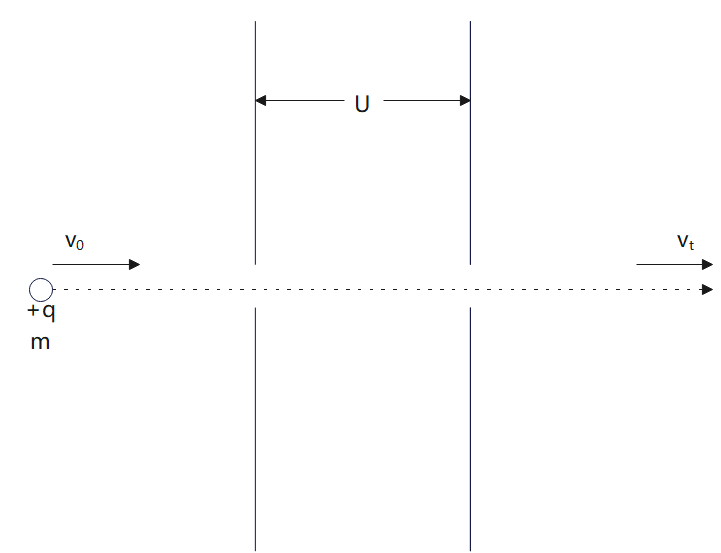
\includegraphics[width=8cm]{11-1}\caption[加速电场示意图]{加速电场示意图}\label{jsdc} \end{figure}
\subsubsection{偏转运动}
受不同电场叠加影响而发生场内偏转时,速度也会随之受到影响.如图\ref{pzdc}\begin{figure}[htp]\centering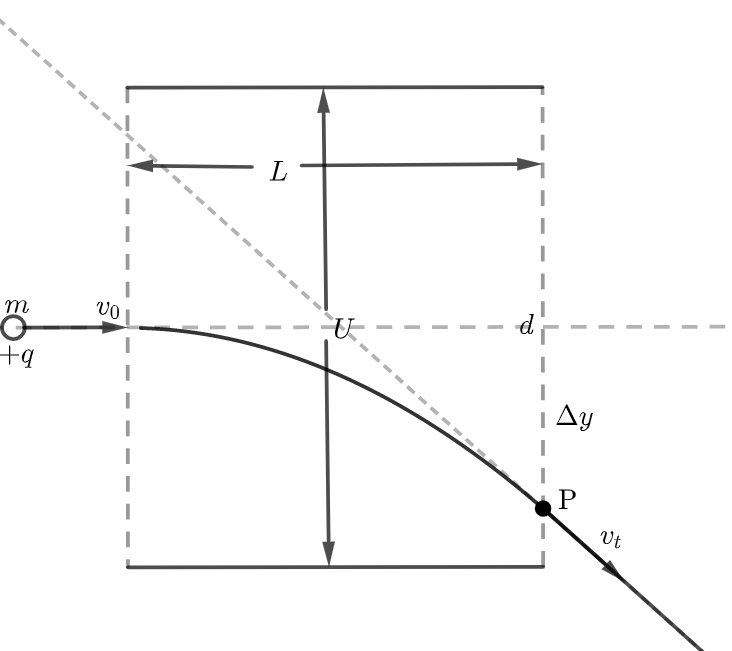
\includegraphics[width=4cm]{11-2}\caption[偏转电场示意图]{偏转电场示意图}\label{pzdc} \end{figure}\newpage


让我们仔细分析一下该偏转电场.两均匀带电板间间隔为$d$,电势差为$U$,长度均为$L$,一质量为$m$、带$+q$的小球以初速度$v_0$沿两板中线进入由两板构成的电容器中(不计重力)且飞出时未触碰到下板,求飞出点P距离中线距离和末速度$v_t$.
\begin{de}射出点与射入点连线与中线夹角$\theta$称为\textbf{电场偏转角};[射出点/与/(射出时速度反向延长线)与(中线)交点/连线]/与中线夹角$\alpha$/称为\textbf{速度偏转角}.\footnote{本句较长且均为\ 与\ 字,因此用/和括号来分割句子以便理解.}\end{de}


在场中的运动是类平抛运动.加速度\begin{equation*}a=\dfrac{qU}{md}\end{equation*} 时间\begin{equation*}
	t=\dfrac{L}{v_0}
\end{equation*}
 故竖直($y$方向)位移\begin{equation*}y=\dfrac{1}{2}\dfrac{qU}{md}({\dfrac{L}{v_0}})^2=\dfrac{qUL^2}{4E_{k}d}\end{equation*}
有\begin{equation*}
	\tan\alpha=\dfrac{v_y}{v_0}=\dfrac{qUL^2}{4E_kdv_0}=\dfrac{qUL^2}{2m{v_0}^3d} 
\end{equation*}
$\tan\theta$的推导十分类似,请读者自己完成推导.
[注意!]$\tan\theta$的结果应为\begin{equation*}\tan\theta=\dfrac{qUL^2}{4mv_0^3d}=\dfrac{1}{2}\tan\alpha\end{equation*}
\subsection{3.2例题}
\paragraph{例1}\qquad a
\subsection{3.2习题}